\chapter{Rendering Surface Geometries using the NMM approach}
\label{chap:diffflssnmm}
In section $\ref{sec:snakegeomrenderings}$ we mentioned that we use the FLSS approach instead of the NMM approach for producing our renderings applied on a snake mesh. The reason for choosing the FLSS approach was that it produces reliable results (according to its evaluation plots as discussed in section $\ref{sec:virtualtestbench}$). Furthermore, the colors of renderings resulting from the NMM approach look purplish compared to those produced by the FLSS approach as shown in figure $\ref{fig:appendixflssvsnmm}$. This figure shows renderings of our snake mesh when using an Elaphe grating produced by the FLSS approach (see figure $\ref{fig:appendixcompflsselaphe}$) and the NMM approach (see figure $\ref{fig:appendixcompnmmlaphe}$). We observe that pixels, which have a bluish color tone in FLSS renderings exhibit a purplish color tone in the corresponding pixels in a NMM rendering. This color-tone shift towards the purple color region for NMM renderings does not correspond to the reality. This issue is directly related to the non-uniform wavelength spectrum sampling of the NMM approach. 

\begin{figure}[H]
  \centering
  \subfigure[FLSS approach]{
    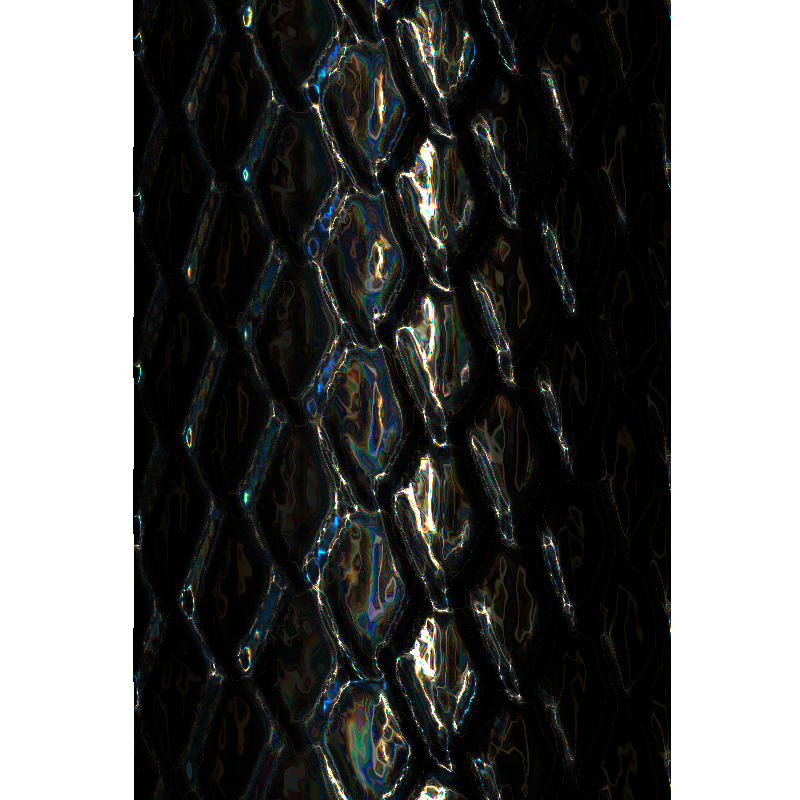
\includegraphics[scale=0.45]{appendix/flss.png}
    \label{fig:appendixcompflsselaphe}
  }
~
  \subfigure[NMM approach]{
    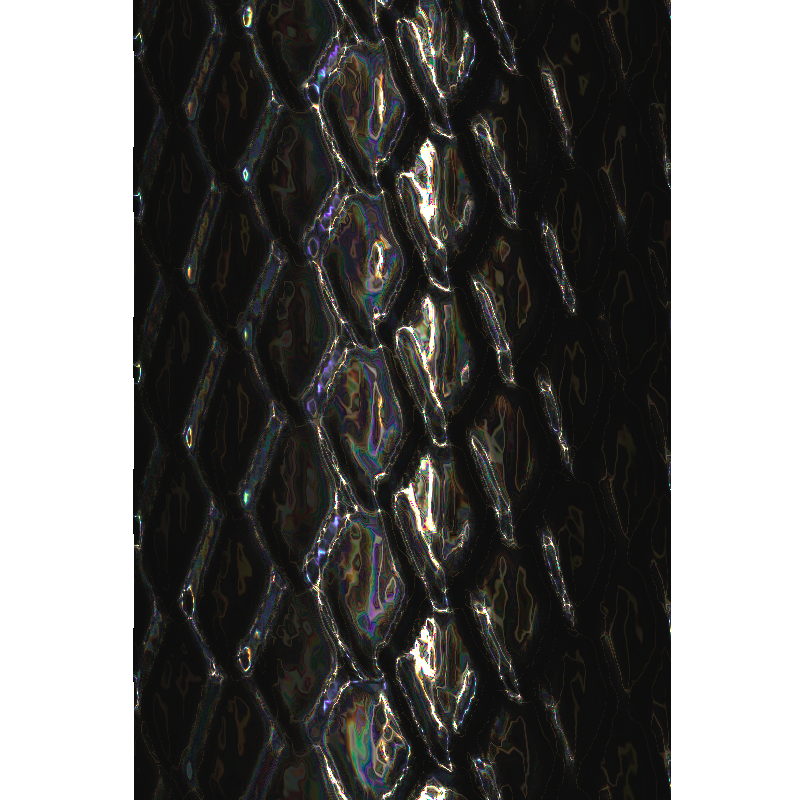
\includegraphics[scale=0.45]{appendix/nmm.png}
    \label{fig:appendixcompnmmlaphe}
  }
~
\caption[Comparing the NMM Approach with the FLSS Approach]{Comparing the FLSS rendering approach with the NMM approach by rendering an Elaphe grating.}
\label{fig:appendixflssvsnmm}
\end{figure}

In order to address this color-tone issue we have to revisit the concept of how we compute the color values in our renderings. For this purpose let us consider the equation $\ref{eq:tristimrad}$ which defines how to compute the CIE XYZ color values. Without loss of generality let us consider the computation of the luminance $Y$ which is equal to:

\begin{align}
Y = \int_{\Lambda}L_\lambda(\omega_r)\overline{y}(\lambda)d\lambda \nonumber
\end{align}

In this formulation we integrate over the whole wavelength spectrum $\Lambda$ for computing the color value for $Y$. However, in the NMM approach we perform a \emph{non-uniform} integration over the wavelength spectrum. Thus, instead of directly integrating over the wavelength spectrum we integrate uniformly over the \emph{minimum} and \emph{maximum} wavenumber (denoted as $N_{min} and N_{max} respectively$) as explained in section $\ref{sec:nmmapproach}$. Therefore, we no longer integrate over the wavelength spectrum rather we integrate over the corresponding wavenumber range $[N_{min}, N_{min}]$. Hence, this depicts a change of integration variables. Unfortunately, I have not taken care of this factor in the NMM approach. And this is why my rendered images produced by the NMM approach look purplish. In the following I describe what this factor is equal to. \\

The wavenumber for a particular wavelength $\lambda$ is equal to

\begin{align}
  k = \frac{2 \pi}{\lambda} \nonumber
\end{align}

The sampling of the the NMM approach performs an integration over infinitesimal wavenumbers $dk$ instead over $d\lambda$. By rearranging the definition of the wavenumber $k$ we can derive the following identity for the wavelength $\lambda$:

\begin{align}
  \lambda = \frac{2 \pi}{k} \nonumber
\end{align}

Thus, the correction factor for changing the integrations variables $d\lambda$ and $dk$ can be computed as the following:

\begin{alignat}{4}
& \frac{d\lambda}{dk} &&= \frac{d}{dk} \left(\frac{2 \pi}{k} \right) = \frac{2 \pi}{k^2}  \nonumber \\
\Rightarrow{} & d\lambda &&= \frac{2 \pi}{k^2} dk \nonumber
\end{alignat}

This will lead us to the final representation for performing an integration over the wavenumber range as defined in equation $\ref{eq:wavenumberintegration}$:
\begin{align}
Y 
&= \int_{\Lambda}L_\lambda(\omega_r)\overline{y}(\lambda)d\lambda \nonumber \\
&= \int_{N_{min}}^{N_{max}} L_k(\omega_r)\overline{y}(k) \frac{2 \pi}{k^2} dk
\label{eq:wavenumberintegration}
\end{align}
